\documentclass[english]{beamer}
\uselanguage{english}

%% PACKAGES %%

\usepackage[utf8]{inputenc}
\usepackage[width=0.8cm, height=1.2cm]{ufcd}
\usepackage{textpos}
\usepackage{chronology} % used for timelines 
\usepackage{graphicx}
\usepackage{tikz}
\usepackage{braket}
\usepackage{scalerel, stackengine, amsmath} % needed for equalhat

\mode<presentation>
{
  \setbeamercovered{invisible}
}

\AtBeginSection[]
{
\begin{frame}<beamer>{Table of contents}
    \tableofcontents[currentsection,currentsubsection]
\end{frame}
}

%% NEW COMMANDS %%

\newcommand{\backupbegin}{
   \newcounter{framenumberappendix}
   \setcounter{framenumberappendix}{\value{framenumber}}
}

\newcommand{\backupend}{
  \addtocounter{framenumberappendix}{-\value{framenumber}}
  \addtocounter{framenumber}{\value{framenumberappendix}} 
}

\newcommand{\portraitpic}[1]{
  \begin{textblock*}{1.6cm}(9.7cm, 0cm)
    \includegraphics[width=\textwidth]{#1}
  \end{textblock*}
}

\newcommand{\picpos}[4]{
  \begin{textblock*}{#1}(#2, #3)
    \includegraphics[width=\textwidth]{#4}
  \end{textblock*}
}

\newcommand\equalhat{\mathrel{\stackon[1.5pt]{=}{\stretchto{%
            \scalerel*[\widthof{=}]{\wedge}{\rule{1ex}{3ex}}}{0.5ex}}}}

\newcommand{\textpos}[4]{
  \begin{textblock*}{#1}(#2, #3)
    #4
  \end{textblock*}
}

\renewcommand{\event}[3][e]{%
  \pgfmathsetlength\xstop{(#2-\theyearstart)*\unit}%
  \ifx #1e%
  \draw[fill=Uni-Blau,draw=none,opacity=0.5]%
  (\xstop, 0) circle (0.5\unit)%
  node[opacity=1,rotate=45,right=.5\unit] {#3};%
  \else%
  \pgfmathsetlength\xstart{(#1-\theyearstart)*\unit}%
  \draw[fill=Uni-Blau,draw=none,opacity=0.5,rounded corners=.2\unit]%
  (\xstart,-.5\unit) rectangle%
  node[opacity=1,rotate=45,right=.5\unit] {#3} (\xstop,.5\unit);%
\fi}%




%% TITLE PAGE %%
\title[Nobelprize 2012]{Nobel prize in physics 2012}
\subtitle{Serge Haroche and David Wineland}
\author[F.~Thielemann]{Fabian~Thielemann}
\institute{Institute of Physics}

\graphicspath{{../Figures/}}

\begin{document}
  \begin{frame}[t]
    \titlepage
  \end{frame}
  
  \section{Introduction}
The Nobel prize in physics 2012 was awarded jointly to the French physicist
Serge Haroche and the American physicist David Wineland.
According to the Nobel jury they received it ``for ground-breaking experimental
methods that enable measuring and manipulation of individual quantum systems''.
Serge Haroche spent most of his life researching at the École Normale Supérieure
in Paris. There he created photon traps, i.e. cavities, in which microwave
photons could be stored up to half a second~\cite{haroche2007QuantumJumps}. To
probe the wave function of the photons, he sent in groups of or single atoms to
see how they would interact with the light. In this way he unveiled many of the
interesting effects of the quantum nature of light. David Wineland spent most of
his scientific life on the other side of the Atlantic, at the National Institute
of Standards and Technology in Boulder, Colorado. His drive was to invent better
methods to slow down and
isolate ions as this allowed frequency measurements of
higher and higher precision. To achieve this, he used sophisticated setups
combining ion traps with high precision lasers. 

But if one of the laureates dedicated his research to photons and the other one
to ions, why did they share the Nobel prize? The answer to this question lies in
the congruence of their methods with respect to quantum mechanics. Haroche was
probing photons with atoms, Wineland examined the energy levels of atoms using
photons, but both were dealing with the same underlying effects of quantum
mechanics. This can be easily seen when one leaves aside their specific physical
objects of study (i.e. photons and ions) and inspects which abstract topics
they were dealing with. Both of them published papers about ``Schrödinger Cat
States''~\cite{brune1992manipulation, monroe1996schrodinger}, bringing to
physical experiment one of the most fundamental thought experiments of early
quantum mechanics. Both conducted experiments on many particle entanglement
~\cite{rauschenbeutel2000step, sackett2000experimental}. Both found ways to
engineer explicitly  non-classical states in their systems~\cite{meekhof1996generation,
deleglise2008reconstruction}. This list could be continued, but the message is
clear: each of them in their own fields found ways to answer fundamental issues
of quantum mechanics experimentally and on their way introduced countless new
methods to the physics community.

The outline of this term paper is as follows: first we will theoretically derive
the phenomenon of Rabi oscillations from the Jaynes-Cummings Hamiltonian, because
both, Haroche and Wineland, used it as a central method in their later
experiments (Sec.~\ref{sec:Theory}) . Then we will have a look at  each of the
laureate's early life and inspect some of their central experiments in order to
get an impression of their experimental creativity and innovation
(Sec.~\ref{sec:Haroche}~and~\ref{sec:Wineland}). A short conclusion will then be
given in Sec.~\ref{sec:Conclusion}.

  \section{Serge Haroche}


\begin{frame}[t]{Serge Haroche: Early life}
  \portraitpic{haroche.jpg}
  \visible<3>{
    \textpos{\linewidth}{0cm}{3cm}{\begin{quote}``I was a very good student,
    immediately at the head of my class in the Lycée Carnot''\end{quote}}
  }
  \visible<6>{\picpos{6cm}{1cm}{2.8cm}{lab_kastler_brossel.jpg}}
  \visible<7>{
    \textpos{\linewidth}{0cm}{3cm}{\begin{quote}``Enthralled by the mysterious beauty of the quantum
          world, it did not take me long to decide that I wanted to become a
        quantum physicist''\end{quote}}
  }

  \begin{minipage}[t][4cm][t]{\textwidth}
    \begin{itemize}
      \item<1-> Born in Casablanca, Morocco
      \item<2-> Parents move to Paris
      \item<4-> École préparatoires at Paris
      \item<5-> Accepted for École normale supérieure (ENS)
    \end{itemize}  
  \end{minipage}
  \begin{minipage}[t][0.2\textheight][t]{\textwidth}
    \begin{chronology}[10]{1940}{2016}{\textwidth}{5cm}
      \visible<1>{\event{1944}{24.02.1944}}
      \visible<2>{\event{1956}{'56}}                  
      \visible<4>{\event{1962}{'62}}                  
      \visible<5,7>{\event[1963]{1967}{'63 -- '67}}
      \visible<>{ \event[1967]{1972}{'67 -- '72}} 
      \visible<>{\event[1972]{1973}{'72 -- '73}}
      \visible<>{\event[1973]{1975}{'73 -- '75}}
      \visible<>{\event[1975]{1982}{'75 -- '82}}
      \visible<>{\event[1982]{2016}{'78-- now}}
    \end{chronology}
  \end{minipage}
\end{frame}

\begin{frame}[t]{Serge Haroche: Scientific Carreer}
  \portraitpic{haroche.jpg}
  \begin{minipage}[t][4.5cm][t]{\textwidth}
    \begin{itemize}
      \item PhD on light dressed atoms in optical pumping
      \item Supervisor: Claude Cohen-Tannoudji
      \picpos{2.5cm}{0.3cm}{1.5cm}{cohen-tannoudji.jpg}
      \picpos{7cm}{3cm}{1.2cm}{dressed_states.pdf}
    \end{itemize}  
  \end{minipage}
  \begin{minipage}[t][0.2\textheight][t]{\textwidth}
    \begin{chronology}[10]{1940}{2016}{\textwidth}{5cm}
      \event[1967]{1972}{'67 -- '72}
    \end{chronology}
  \end{minipage}
\end{frame}

\begin{frame}[t]{Serge Haroche: Scientific Carreer}
  \portraitpic{haroche.jpg}
  \visible<1>{
    \picpos{2.8cm}{1cm}{1.5cm}{arthur_schawlow_np.jpg}
    \picpos{2.8cm}{5cm}{1.5cm}{ted_haensch.jpg}
  }
  \visible<2>{\textpos{\linewidth}{0cm}{2.5cm}{\begin{quote}``After a few weeks in
  Stanford Art gave me a lab room and a pulsed dye laser and told me it was up
  to me to find something interesting to do with it.''\end{quote}}}
  \visible<3>{\picpos{9cm}{0.5cm}{1.5cm}{SH_quantum_beats_title.pdf}}
  \visible<4>{\picpos{3.7cm}{0.5cm}{3cm}{v_type_quantum_beats.pdf}}
  \visible<4>{\begin{textblock*}{3cm}(0.5cm,2.5cm)V-type\end{textblock*}}
  \visible<4>{\picpos{4.8cm}{5.5cm}{3cm}{lambda_type_quantum_beats.pdf}}
  \visible<4>{\begin{textblock*}{3cm}(5.5cm,2.5cm)$\Lambda$-type\end{textblock*}}
  \visible<5->{\picpos{3.7cm}{0.5cm}{2cm}{SH_quantum_beats_plot.pdf}}
  %\visible<>{\picpos{5cm}{4.8cm}{2.5cm}{SH_quantum_beats_setup.pdf}}
  \visible<5>{\picpos{5.5cm}{4.8cm}{2.8cm}{SH_quantum_beats_results.pdf}}
  \begin{minipage}[t][4.5cm][t]{\textwidth-1.9cm}
    \begin{itemize}
      \setlength\itemsep{0.9em}
      \item Postdoc at Arthur Schawlows Lab in Stanford
      \item<3-> Observation of quantum beats in Cs vapor
      \begin{quote}\end{quote}
    \end{itemize}  
  \end{minipage}
  \begin{minipage}[t][0.2\textheight][t]{\textwidth}
    \visible<1-3>{
    \begin{chronology}[10]{1940}{2016}{\textwidth}{5cm}
      \event[1972]{1973}{'72 -- '73}
    \end{chronology}
  }
  \end{minipage}
\end{frame}

\begin{frame}[t]{Serge Haroche: Scientific Carreer}
  \portraitpic{haroche}
  \begin{minipage}[t][4.5cm][t]{\textwidth-1.9cm}
    \begin{itemize}
      \setlength\itemsep{0.9em}
      \item Budget and laboratory at ENS: Beginning of experimental studies of Rydberg atoms 
      \item<2-> Full professor at Université Paris VI
      \item<3-> Professorship and research at Yale {\em and} ENS
      \item<4-> Professor at Collège de France
      \item<5-> Gold medal of the Centre national de la récherche scientifique
        (CNRS)
    \end{itemize}  
  \end{minipage}
  \begin{minipage}[t][0.2\textheight][t]{\textwidth}
    \begin{chronology}[10]{1940}{2016}{\textwidth}{5cm}
      \visible<1>{\event{1973}{'73}}
      \visible<2>{\event{1975}{'75}}
      \visible<3>{\event[1984]{1993}{'84 -- '93}}
      \visible<4>{\event{1999}{'99}}
      \visible<5>{\event{2009}{'09}}
    \end{chronology}
  \end{minipage}
\end{frame}


\begin{frame}[t]{Serge Haroche: CQED}
  \portraitpic{haroche}
  \visible<1>{\picpos{4cm}{.5cm}{1.5cm}{atom_in_cavity.pdf}}
  \visible<2>{\picpos{4cm}{.5cm}{1.5cm}{atom_in_cavity_res.pdf}}
  \visible<2>{\begin{textblock*}{5.5cm}(5cm,2.5cm)Resonant case $$\Gamma_{res} =
    \Gamma_0 \, \frac{3Q\lambda^3}{4\pi^2V}$$ $\rightarrow$ enhanced spontaneous
    emission\end{textblock*}}
  \visible<3>{\picpos{9cm}{0.5cm}{2.5cm}{SH_cavity_enhanced_em_title.pdf}}
  \visible<4->{
    \picpos{5cm}{0.5cm}{1.5cm}{SH_cavity_enhanced_em_setup.pdf}
    \textpos{3cm}{0.3cm}{3.6cm}{\small 23S}
  }
  \visible<4>{\textpos{3cm}{5.55cm}{4.7cm}{\small 23S or 22P?}}
  \visible<5>{\picpos{4cm}{5.55cm}{2.5cm}{SH_cavity_enhanced_em_results.pdf}}
    
  \begin{minipage}[t][4.5cm][t]{\textwidth-1.5cm}
    \begin{itemize}
      \item Cavity QED (CQED): what happens to atoms in cavities?
    \end{itemize}  
  \end{minipage}
  \begin{minipage}[t][0.2\textheight][t]{\textwidth}
    \visible<3>{
    \begin{chronology}[10]{1940}{2016}{\textwidth}{2cm}
      \visible<3>{\event{1983}{'83}}
      \visible<>{\event{1999}{'99 -- '99}} %this will never be visible, just
        % takes care of spacing
    \end{chronology}
  }
  \end{minipage}
\end{frame}

\begin{frame}[t]{Serge Haroche: CQED}
  \portraitpic{haroche}
  \visible<1>{\picpos{4cm}{.5cm}{1.5cm}{atom_in_cavity.pdf}}
  \visible<2>{\picpos{4cm}{.5cm}{1.5cm}{atom_in_cavity_cut.pdf}}
  \visible<2>{
    \begin{textblock*}{5.5cm}(5cm,2.8cm) Polarization dependend ``cut-off'' of
      vacuum modes \end{textblock*}
    \textpos{5.5cm}{5.3cm}{3.9cm}{$\rightarrow$}
    \textpos{5.5cm}{5.75cm}{3.75cm}{supression of spontaneous
    emission}
    }
  \visible<3>{\picpos{9cm}{0.5cm}{1.5cm}{SH_supression_spont_em_title.pdf}}
  \visible<4->{
    \picpos{5.5cm}{0.5cm}{2cm}{SH_supressed_spont_em_setup.jpg}
  }
  \visible<4-5,7-8>{\picpos{4cm}{6.3cm}{3cm}{SH_supression_spont_em_scheme.pdf}}
  \visible<6>{\picpos{6cm}{6.3cm}{3cm}{SH_supression_spont_em_scheme2.pdf}}
  \visible<5>{
    \picpos{5.5cm}{0.5cm}{2cm}{SH_supressed_spont_em_setup_1.pdf}
    \textpos{2.5cm}{-0.4cm}{4.1cm}{\scriptsize Excitation to 7P$_{3/2}$ and decay
      to 5D$_{3/2}$}
    }
  \visible<6>{
    \picpos{5.5cm}{0.5cm}{2cm}{SH_supressed_spont_em_setup_2.pdf}
    \textpos{3.6cm}{2.5cm}{6cm}{\scriptsize Flight through cavity\\ $\approx
  13$ natural lifetimes}
    }
  \visible<7>{
    \picpos{5.5cm}{0.5cm}{2cm}{SH_supressed_spont_em_setup_3.pdf}
    \textpos{3cm}{3.8cm}{5.65cm}{\scriptsize Excitation to 26F}
    }
  \visible<8>{
    \picpos{5.5cm}{0.5cm}{2cm}{SH_supressed_spont_em_setup_4.pdf}
    \textpos{3cm}{4.1cm}{5.65cm}{\scriptsize Ionization detection\\ of 26F}
    }
  \visible<9>{\picpos{4cm}{6cm}{2.5cm}{SH_supression_spont_em_results.pdf}}
    
  \begin{minipage}[t][4.5cm][t]{\textwidth-1.5cm}
    \begin{itemize}
      \item Cavity QED (CQED): what happens to atoms in cavities?
    \end{itemize}  
  \end{minipage}
  \begin{minipage}[t][0.2\textheight][t]{\textwidth}
    \visible<3>{
    \begin{chronology}[10]{1940}{2016}{\textwidth}{2cm}
      \visible<3>{\event{1987}{'87}}
      \visible<>{\event{1999}{'99 -- '99}} %this will never be visible, just
        % takes care of spacing
    \end{chronology}
  }
  \end{minipage}
\end{frame}

\begin{frame}[t]{Serge Haroche: QND Measurement}
  \portraitpic{haroche}
  \visible<2>{\picpos{6cm}{2cm}{2.9cm}{SH_single_photon_detection_title.pdf}}
  \visible<3>{\picpos{8cm}{1cm}{3.9cm}{sh_super_high_q_title.pdf}}
  \begin{minipage}[t][4.5cm][t]{\textwidth-1.5cm}
    \begin{itemize}
      \item Quantum non-demolition (QND) measurement: can we observe photons
        without destroying them?
      \item<2-> Probe photon field with  slightly off-resonant Rydberg atom
      \item<3-> Breakthrough: super-high-Q cavity to store photons for
        $\approx\,$0.1\,s $\equalhat$ 30000\,km
    \end{itemize}  
  \end{minipage}
  \begin{minipage}[t][0.2\textheight][t]{\textwidth}
    \visible<2-3>{
    \begin{chronology}[10]{1940}{2016}{\textwidth}{2cm}
      \visible<2>{\event{1999}{'99}}
      \visible<3>{\event{2006}{'06}}
      \visible<>{\event{1999}{'99 -- '99}} %this will never be visible, just
        % takes care of spacing
    \end{chronology}
  }
  \end{minipage}
\end{frame}

\begin{frame}[t]{Serge Haroche: QND Measurement}
  \portraitpic{haroche}
  \visible<1->{\picpos{7cm}{0cm}{1cm}{sh_photon_detection_background.pdf}}
  \visible<1->{\picpos{5cm}{7cm}{3cm}{rabi_cycle.pdf}}
  
  \visible<2>{\picpos{7cm}{0cm}{1cm}{sh_photon_detection_1.pdf}}
  \visible<2>{\picpos{5cm}{7cm}{3cm}{rabi_cycle_1.pdf}}
  \visible<2>{\textpos{4cm}{0.6cm}{4.8cm}{\small creation of Rydberg state
  $\ket{e}=\ket{51}$}} 

  \visible<3>{\picpos{7cm}{0cm}{1cm}{sh_photon_detection_2.pdf}}
  \visible<3>{\picpos{5cm}{7cm}{3cm}{rabi_cycle_2.pdf}}
  \visible<3>{\textpos{4cm}{1.2cm}{4.8cm}{\small $\pi /2$-pulse}} 
  
  \visible<4>{\picpos{7cm}{0cm}{1cm}{sh_photon_detection_3.pdf}}
  \visible<4>{\textpos{6cm}{1.2cm}{4.8cm}{\small Rabi induced phase shift $ \Phi=
\begin{cases} 0 & \text{if no photon}\\ \pi  & \text{if one photon} \end{cases}$ }} 
  
  \visible<5>{\picpos{7cm}{0cm}{1cm}{sh_photon_detection_4.pdf}}
  \visible<5>{\textpos{4cm}{1.2cm}{4.8cm}{\small $\pi /2$-pulse $\ket{\psi} =
\begin{cases} \ket{g} & \text{if no photon}\\ \ket{e}  & \text{if one photon} \end{cases}$}} 
  
  \visible<6>{\picpos{7cm}{0cm}{1cm}{sh_photon_detection_5.pdf}}
  \visible<6>{\textpos{4cm}{1.7cm}{4.8cm}{\small ionization detection\\ $\ket{g}$
  or $\ket{e}$}} 

  \begin{minipage}[t][4.5cm][t]{\textwidth-1.5cm}
    \begin{itemize}
      \item Quantum non-demolition measurement scheme
    \end{itemize}  
  \end{minipage}
  \begin{minipage}[t][0.2\textheight][t]{\textwidth}
    \visible<>{
    \begin{chronology}[10]{1940}{2016}{\textwidth}{2cm}
      \visible<2>{\event{1999}{'99}}
      \visible<3>{\event{2006}{'06}}
      \visible<>{\event{1999}{'99 -- '99}} %this will never be visible, just
        % takes care of spacing
    \end{chronology}
  }
  \end{minipage}
\end{frame}

\begin{frame}[t]{Serge Haroche: QND Photon counting}
  \portraitpic{haroche}
  \visible<1>{\picpos{8cm}{0.5cm}{1.5cm}{SH_photon_quantum_jumps_title.pdf}}
  \visible<2>{\picpos{6cm}{0.5cm}{1.5cm}{SH_photon_quantum_jumps_results.pdf}}
  \visible<2>{\textpos{\textwidth}{0.5cm}{5.5cm}{$\rightarrow$ photon ``born'' in
  vacuum survives in cavity for 0.5\,s, measured by several hundreds of atoms}}

  \begin{minipage}[t][4.5cm][t]{\textwidth-1.5cm}
    \begin{itemize}
      \item Black body photon quantum jumps
    \end{itemize}  
  \end{minipage}
  \begin{minipage}[t][0.2\textheight][t]{\textwidth}
    \visible<1>{
    \begin{chronology}[10]{1940}{2016}{\textwidth}{2cm}
      \visible<1>{\event{2007}{'07}}
      \visible<>{\event{1999}{'99 -- '99}} %this will never be visible, just
        % takes care of spacing
    \end{chronology}
  }
  \end{minipage}
\end{frame}

\begin{frame}[t]{Serge Haroche: QND Photon counting}
  \portraitpic{haroche}
  \visible<1>{\picpos{8cm}{0.5cm}{1.5cm}{SH_field_state_collapse_title.pdf}}
  \visible<2>{\picpos{9cm}{0.5cm}{1.5cm}{SH_field_state_collapse_results.pdf}}
  \visible<2>{\textpos{\textwidth}{0.5cm}{5.5cm}{$\rightarrow$ wavefunction collapse from
  quantum fluctuation to ``classical'' single mode occupation}}

  \begin{minipage}[t][4.5cm][t]{\textwidth-1.5cm}
    \begin{itemize}
      \item Photon number wavefunction in cavity
    \end{itemize}  
  \end{minipage}
  \begin{minipage}[t][0.2\textheight][t]{\textwidth}
    \visible<1>{
    \begin{chronology}[10]{1940}{2016}{\textwidth}{2cm}
      \visible<1>{\event{2007}{'07}}
      \visible<>{\event{1999}{'99 -- '99}} %this will never be visible, just
        % takes care of spacing
    \end{chronology}
  }
  \end{minipage}
\end{frame}

  \section{David Wineland}

\begin{frame}[t]{David Wineland: In a nutshell}
  \portraitpic{wineland.jpg}
  \vspace{3cm}
  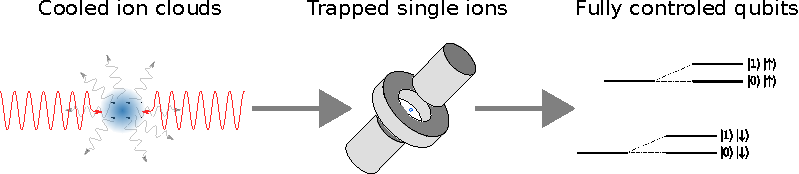
\includegraphics[width=\textwidth]{dw_nutshell.pdf}
\end{frame}

\begin{frame}[t]{David Wineland: Early life}
  \portraitpic{wineland.jpg}
  \visible<3>{
    \textpos{\linewidth}{0cm}{3cm}{\begin{quote}``I knew I was destined to go to
    college and I always kept up my grades to be able to do that''\end{quote}}
  }
  \visible<6>{
    \textpos{\linewidth}{0cm}{3cm}{\begin{quote}``Because I respected my
        classical mechanics teacher so
    much, I asked him about places to apply for graduate school. He recommended
  Harvard, so I applied there.''\end{quote}}
  }
  \begin{minipage}[t][4.5cm][t]{\textwidth-1.5cm}
    \begin{itemize}
      \item<1-> Born near Milwaukee, Wisconsin
      \item<2-> Parents moved to Sacramento, California
      \item<4-> Math Major at University of California, Davis
      \item<5-> Transfer to Berkeley as Physics Major
    \end{itemize}  
  \end{minipage}

  \begin{minipage}[t][0.2\textheight][t]{\textwidth}
    \begin{chronology}[10]{1940}{2016}{\textwidth}{5cm}
      \visible<1>{\event{1944}{24.02.1944}}
      \visible<2>{\event{1947}{'47}}
      \visible<4>{\event{1961}{'61}}
      \visible<5>{\event[1962]{1965}{'62 -- '65}}
    \end{chronology}
  \end{minipage}
\end{frame}

\begin{frame}[t]{David Wineland: Scientific Carreer}
  \portraitpic{wineland.jpg}
  \visible<1>{
    \picpos{6.5cm}{1cm}{1.5cm}{norman_ramsey_group_np.jpg}
  }
  \begin{minipage}[t][4.5cm][t]{\textwidth-1.5cm}
    \begin{itemize}
      \item Master and PhD at Norman Ramseys group in Harvard
      \item<2> Spectroscopy of hyperfine levels of Deuterium
    \end{itemize}  
  \end{minipage}
  \begin{minipage}[t][0.2\textheight][t]{\textwidth}
    \begin{chronology}[10]{1940}{2016}{\textwidth}{5cm}
      \event[1965]{1970}{'65 -- '70}
    \end{chronology}
  \end{minipage}
\end{frame}

\begin{frame}[t]{David Wineland: Scientific Carreer}
  \portraitpic{wineland.jpg}
  \visible<1>{
    \picpos{3cm}{1cm}{1.5cm}{hans_dehmelt_np.jpg}
  }
  \visible<2>{
    \picpos{8cm}{1cm}{2cm}{monoelectron_title.jpg}
  }
  \visible<3>{
    \picpos{8cm}{0.5cm}{2cm}{dw_penning_trap.pdf}
  }
  \visible<4->{
    \picpos{9cm}{1cm}{2.5cm}{dw_monoelectron_plot.pdf}
  }
  \visible<5>{
    \picpos{9cm}{1cm}{2.5cm}{dw_monoelectron_plot1.pdf}
  }
  \visible<6>{
    \picpos{9cm}{1cm}{2.5cm}{dw_monoelectron_plot2.pdf}
  }
  \visible<7>{
    \picpos{9cm}{1cm}{2.5cm}{dw_monoelectron_plot3.pdf}
  }
  \begin{minipage}[t][4.5cm][t]{\textwidth-1.5cm}
    \begin{itemize}
      \item Postdoc in Hans Dehmelts group in Washington
      \item<2-> Trapping single electrons in a Penning trap
    \end{itemize}  
  \end{minipage}
  \begin{minipage}[t][0.2\textheight][t]{\textwidth}
    \visible<1-2>{
      \begin{chronology}[10]{1940}{2016}{\textwidth}{5cm}
        \visible<1>{\event[1970]{1975}{'70 -- '75}}
        \visible<2>{\event{1973}{'73}}
      \end{chronology}
    }
  \end{minipage}
\end{frame}

\begin{frame}[t, noframenumbering]{David Wineland: Scientific Carreer}
  \portraitpic{wineland.jpg}
  \visible<1->{
    \picpos{7cm}{1cm}{2.5cm}{doppler_cooling.pdf}
  }
  \begin{minipage}[t][4.5cm][t]{\textwidth-1.5cm} %TODO Citation of paper
    \begin{itemize}
      \item Postdoc in Hans Dehmelts group in Washington
      \item Idea of laser cooling of ions (Doppler cooling)
    \end{itemize}  
  \end{minipage}
  \begin{minipage}[t][0.2\textheight][t]{\textwidth}
    \begin{chronology}[10]{1940}{2016}{\textwidth}{5cm}
      \visible<>{\event[1970]{1975}{'70 -- '75}}
      \visible<1>{\event{1975}{'75}}
    \end{chronology}
  \end{minipage}
\end{frame}

\begin{frame}[t]{David Wineland: Scientific Carreer}
  \portraitpic{wineland.jpg}
  \visible<2->{
    \picpos{4.5cm}{1cm}{2.1cm}{dw_cs_clock.jpg}
  }
  \begin{minipage}[t][4.5cm][t]{\textwidth-1.5cm} 
    \begin{itemize}
      \item Position at the time and frequency division of the national bureau
        of standards (NBS, later NIST)

      \item In charge of setting up a working Cesium clock
    \end{itemize}  
  \end{minipage}
  \begin{minipage}[t][0.2\textheight][t]{\textwidth}
    \begin{chronology}[10]{1940}{2016}{\textwidth}{5cm}
      \visible<1>{\event[1975]{1977}{'75 -- '77}}
    \end{chronology}
  \end{minipage}
\end{frame}

\begin{frame}[t]{David Wineland: Scientific Carreer}
  \portraitpic{wineland.jpg}
  \visible<1>{
    \picpos{6cm}{1cm}{1.5cm}{dw_group_79.jpg}
  }
  
  \visible<3>{
    \picpos{9cm}{1cm}{2.5cm}{dw_doppler_cooling_title_full.jpg}
  }

  \visible<4-5>{
    \picpos{5.5cm}{0.5cm}{3cm}{dw_laser_cooling_ions_setup.pdf}
  }

  \visible<5>{
    \picpos{5.5cm}{6cm}{3.5cm}{dw_laser_cooling_ions_plot.pdf}
  }

  \visible<6>{
    \picpos{9cm}{1cm}{2.5cm}{dw_doppler_cooling_title.jpg}
  }
  
  \visible<6>{
    \picpos{9cm}{1cm}{4.8cm}{dehmelt_toschek_cooling_title.jpg}
  }
   
  \visible<2>{
    \textpos{\linewidth}{0cm}{3cm}{\begin{quote}``I knew that we had competition
    because I was aware that Dehmelt had taken a sabbatical to work in Peter
Toschek's lab in Heidelberg, with the same goal of demonstrating cooling.''\end{quote}}
  }
  \begin{minipage}[t][4.5cm][t]{\textwidth-1.5cm}
    \begin{itemize}
      \item<1-> Own group at NBS to research trapped ions and lasers
      \item<2-> Taking up the earlier idea of Doppler cooling
    \end{itemize}  
  \end{minipage}
  \begin{minipage}[t][0.2\textheight][t]{\textwidth}
    \visible<1>{
      \begin{chronology}[10]{1940}{2016}{\textwidth}{5cm}
        \event[1977]{2016}{'77 -- '16 }
      \end{chronology}
    }
  \end{minipage}
\end{frame}

\begin{frame}[c]
  \begin{center}
      \Large Trapped single electrons and cooled down ion clouds, what is next?  
  \end{center}
\end{frame}

\begin{frame}[t]{David Wineland: Research}
  \portraitpic{wineland.jpg}
  \visible<1,5>{
    \picpos{9cm}{.7cm}{1.7cm}{dw_single_mg_title.pdf}
  }
  \visible<2-4>{
    \picpos{8cm}{1cm}{1.5cm}{dw_single_mg_plot.pdf}
  }
  \visible<3>{\picpos{8cm}{1cm}{1.5cm}{dw_single_mg_plot1.pdf}}
  \visible<4>{\picpos{8cm}{1cm}{1.5cm}{dw_single_mg_plot2.pdf}}
  \visible<5>{\picpos{9cm}{.7cm}{4.1cm}{dehmelt_mono_ion_title.pdf}}

  \begin{minipage}[t][4.5cm][t]{\textwidth-1.5cm}
    \begin{itemize}
      \item Trapping of single ions
    \end{itemize}  
  \end{minipage}
  \begin{minipage}[t][0.2\textheight][t]{\textwidth}
    \visible<1>{
      \begin{chronology}[10]{1940}{2016}{\textwidth}{5cm}
        \event{1981}{'81 }
        \visible<>{\event{1999}{'99 -- '99}} %this will never be visible, just
      \end{chronology}
    }
  \end{minipage}
\end{frame}

\begin{frame}[t]{David Wineland: Ion Quantum Jumps}
  \portraitpic{wineland.jpg}

  \visible<1>{
    \picpos{8cm}{0.5cm}{1.9cm}{DW_quantum_jumps_title.pdf}
  }

  \visible<2>{\picpos{7.5cm}{0cm}{1.9cm}{dw_quantum_jumps_scheme0.pdf}}
  \visible<3>{\picpos{7.5cm}{0cm}{1.9cm}{dw_quantum_jumps_scheme1.pdf}}
  \visible<4>{\picpos{7.5cm}{0cm}{1.9cm}{dw_quantum_jumps_scheme2.pdf}}
  \visible<4>{\textpos{5cm}{7.5cm}{4.5cm}{\small fluorescence only when ion occupies
    ground state}}
  \visible<5>{\picpos{7.5cm}{0cm}{1.9cm}{dw_quantum_jumps_scheme_level.pdf}}
  
  \visible<5>{
    \picpos{7cm}{2.8cm}{3cm}{DW_quantum_jumps_results.pdf}
    \textpos{6cm}{3cm}{5.5cm}{\small $\rightarrow$ quantum jumps between ground
    and excited state}
  }
  \begin{minipage}[t][4.5cm][t]{\textwidth-1.5cm}
    \begin{itemize}
      \item Quantum jumps of an ions electron shell
    \end{itemize}  
  \end{minipage}
  \begin{minipage}[t][0.2\textheight][t]{\textwidth}
    \visible<1>{
      \begin{chronology}[10]{1940}{2016}{\textwidth}{5cm}
        \event{1986}{'86 }
        \visible<>{\event{1999}{'99 -- '99}} %this will never be visible, just
      \end{chronology}
    }
  \end{minipage}
\end{frame}

\begin{frame}[t]{David Wineland: Research}
  \portraitpic{wineland.jpg}
  \visible<1>{
    \picpos{8cm}{0.5cm}{1.9cm}{dw_recoilless_single_ion_title.pdf}
  }

  %\visible<2>{
  %  \picpos{\textwidth}{0cm}{1.9cm}{dw_quantized_motion_plot.pdf}
  %}
  \begin{minipage}[t][4.5cm][t]{\textwidth-1.5cm}
    \begin{itemize}
      \item Quantized motional states of the ion in the trap can be resolved
        with a tunable laser
    \end{itemize}  
  \end{minipage}
  \begin{minipage}[t][0.2\textheight][t]{\textwidth}
    \visible<1>{
      \begin{chronology}[10]{1940}{2016}{\textwidth}{5cm}
        \event{1987}{'87 }
        \visible<>{\event{1999}{'99 -- '99}} %this will never be visible, just
      \end{chronology}
    }
  \end{minipage}
\end{frame}

\begin{frame}[t]{David Wineland: Research}
  \portraitpic{wineland.jpg}
  \visible<1>{
    \picpos{8cm}{0.5cm}{1.9cm}{DW_zero_point_energy_title.pdf}
  }
  \visible<2>{
    \picpos{\textwidth}{0cm}{1.9cm}{sideband_cooling_scheme_2_0.pdf}
  }
  \visible<3>{
    \picpos{\textwidth}{0cm}{1.9cm}{sideband_cooling_scheme_3.pdf}
  }
  \visible<4>{
    \picpos{\textwidth}{0cm}{1.9cm}{sideband_cooling_scheme_4.pdf}
  }
  \visible<5>{
    \picpos{\textwidth}{0cm}{1.9cm}{sideband_cooling_scheme_5.pdf}
  }
  \visible<6>{
    \picpos{\textwidth}{0cm}{1.9cm}{sideband_cooling_scheme_6.pdf}
  }
  \visible<7>{
    \picpos{\textwidth}{0cm}{1.9cm}{sideband_cooling_scheme_7.pdf}
    \textpos{4cm}{7.5cm}{6cm}{\small $\rightarrow$ Atom cooled to motional ground state}
  }
  \visible<2->{
    \picpos{\textwidth}{0cm}{1.9cm}{sideband_cooling_scheme_states.pdf}
  }
  \begin{minipage}[t][4.5cm][t]{\textwidth-1.5cm}
    \begin{itemize}
      \item Resolved sideband cooling to motional ground state
    \end{itemize}  
  \end{minipage}
  \begin{minipage}[t][0.2\textheight][t]{\textwidth}
    \visible<1>{
      \begin{chronology}[10]{1940}{2016}{\textwidth}{5cm}
      \visible<>{\event{1999}{'99 -- '99}} %this will never be visible, just
        \event{1989}{'89}
      \end{chronology}
    }
  \end{minipage}
\end{frame}


\begin{frame}[t]{David Wineland: Quantum Logic Gate}
  \portraitpic{wineland.jpg}
  \visible<1>{\picpos{9cm}{0.5cm}{1.5cm}{DW_cnot_gate_title.pdf}}
  \visible<2->{\picpos{5cm}{0.8cm}{2.5cm}{qubits.pdf}}
  \visible<2>{\textpos{5cm}{6.4cm}{3.5cm}{internal qubit
    $\begin{cases}\ket{\uparrow} \\ \ket{\downarrow}\end{cases}$}}
  \visible<2>{\textpos{5cm}{7cm}{5cm}{trap qubit
    $\begin{cases}\ket{0} \\ \ket{1}\end{cases}$}}
  \visible<3-5>{\textpos{6cm}{5.4cm}{3.8cm}{\begin{itemize}\item 4 possible pure
      states \item superposition states can be engineered by laser
pulses \item<5> basic logic operations possible\end{itemize}}}
  \visible<4>{\textpos{8cm}{0.8cm}{6cm}{$\ket{0}\ket{\downarrow}
  \xrightarrow[\text{blue sideband}]{\hspace{0.5cm}\pi/2\text{-pulse on}\hspace{0.5cm}}
  \frac{1}{\sqrt{2}}\left( \ket{0}\ket{\downarrow} + \ket{1}\ket{\uparrow}\right)$}}

  \visible<4>{\picpos{5cm}{0.8cm}{2.5cm}{qubits_arrow.pdf}}
  \begin{minipage}[t][4.5cm][t]{\textwidth-1.7cm}
    \begin{itemize}
      \item Use of trapped ion to store and manipulate two qubits
    \end{itemize}  
  \end{minipage}
  \begin{minipage}[t][0.2\textheight][t]{\textwidth}
    \visible<1>{
      \begin{chronology}[10]{1940}{2016}{\textwidth}{5cm}
        \event{1996}{'95 }
        \visible<>{\event{1999}{'99 -- '99}} %this will never be visible, just
      \end{chronology}
    }
  \end{minipage}
\end{frame}

\begin{frame}[t]{David Wineland: Quantum Logic Gate}
  \portraitpic{wineland.jpg}
  \visible<2->{\picpos{4cm}{0.8cm}{2.8cm}{controled_not.pdf}}
  \visible<3->{\picpos{6cm}{5.2cm}{2.8cm}{DW_cnot_gate_truthtable.pdf}}

  \begin{minipage}[t][4.5cm][t]{\textwidth-1.7cm}
    \begin{itemize}
      \item Controled NOT gate (CNOT): flip target qubit ($\ket{\uparrow}$ or
        $\ket{\downarrow}$) only if control qubit ($\ket{0}$ or $\ket{1}$) is $\ket{1}$
    \end{itemize}  
  \end{minipage}
  \begin{minipage}[t][0.2\textheight][t]{\textwidth}
    \visible<>{
      \begin{chronology}[10]{1940}{2016}{\textwidth}{5cm}
        %\event{1996}{'95 }
        \visible<>{\event{1999}{'99 -- '99}} %this will never be visible, just
      \end{chronology}
    }
  \end{minipage}
\end{frame}

  \begin{frame}[t]{Conclusion}
  \visible<1>{
    \picpos{.3\linewidth}{0cm}{3cm}{tunable_laser.jpg}
    \picpos{.3\linewidth}{.3\linewidth+0.2cm}{2.5cm}{ion_trap.pdf}
    \picpos{.3\linewidth}{0.6\linewidth+0.4cm}{3cm}{cavity_photo.jpg}
  }
  \begin{itemize}
    \item<1-> Possible only with tunable lasers, ion traps and semiconductor
      technology
    \item<2-> observation of single particles for fundamental insight into
      principles of quantum mechanics:
      \begin{itemize}
        \item quantum jumps
        \item entangled states
        \item decoherence processes
      \end{itemize}
    \item<3-> possible applications in quantum computing (e.g. Q20:20)
    \item<4> a decent set of experimental methods for future physicists to play
      with
  \end{itemize}
\end{frame}

\begin{frame}[t]{Take home message}
  \begin{center}
    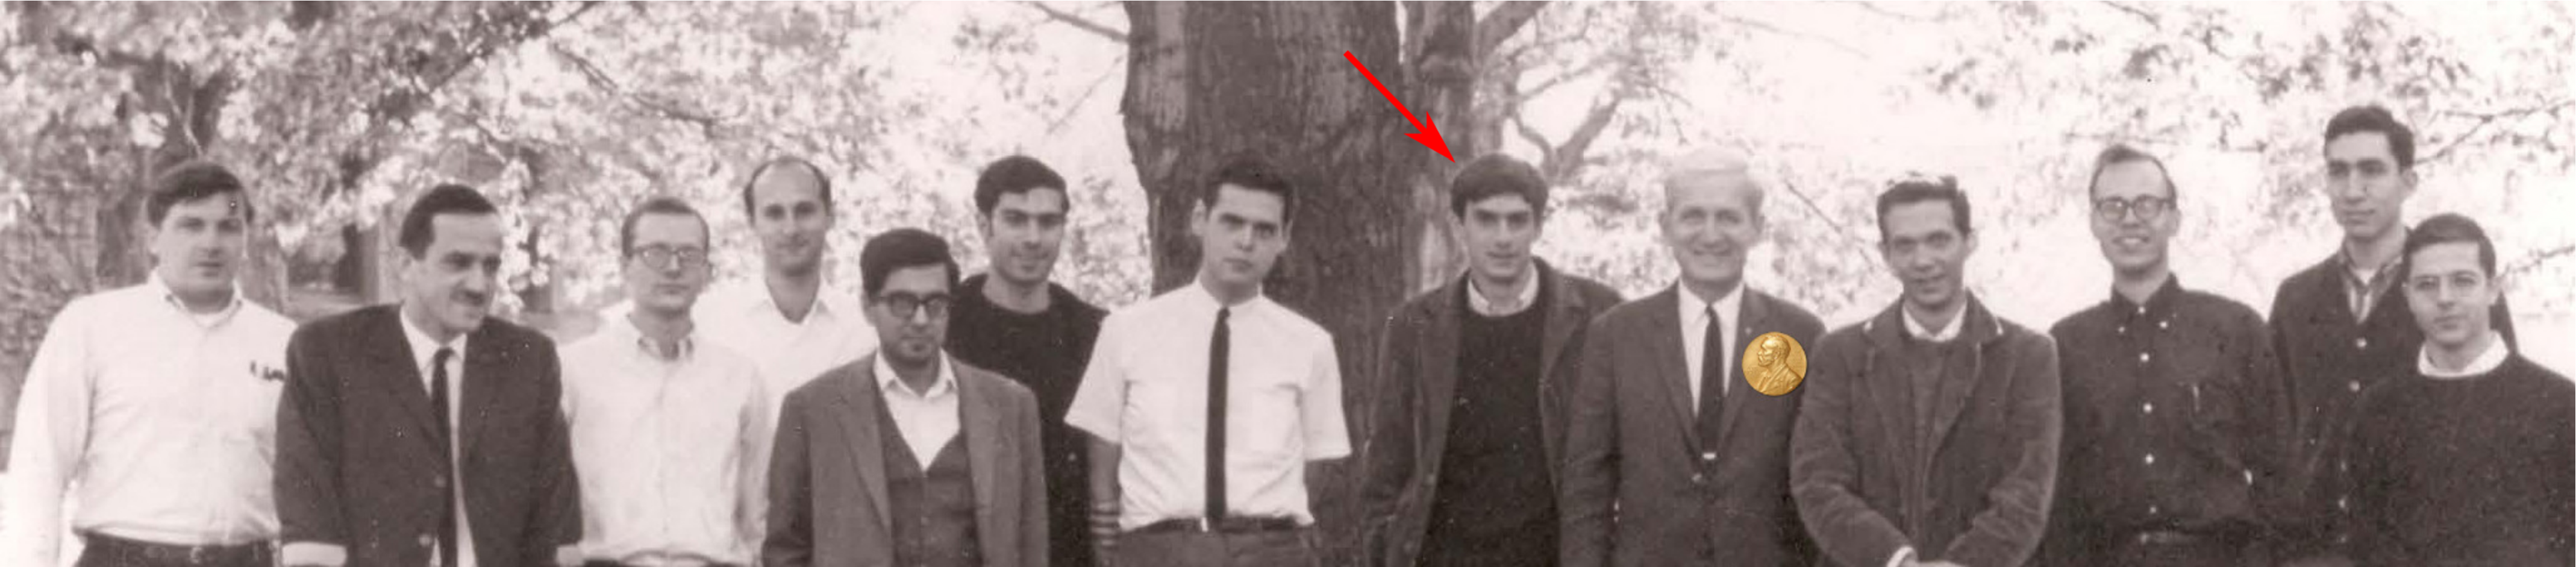
\includegraphics[width=0.9\textwidth]{norman_ramsey_group_arrow.pdf}\\
    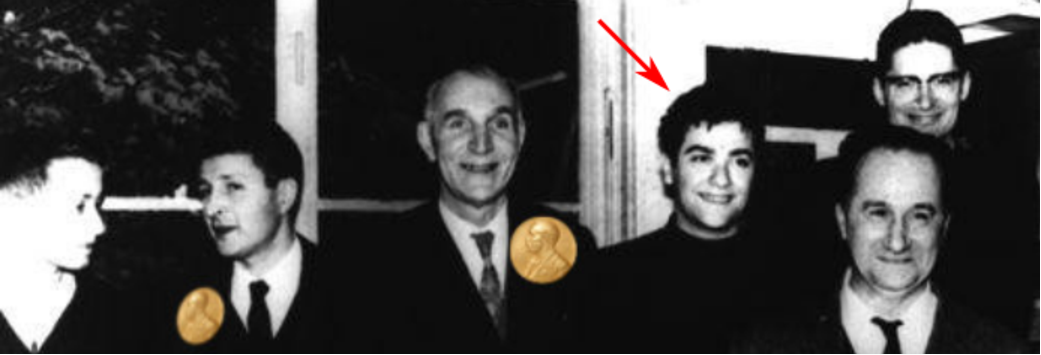
\includegraphics[width=0.9\textwidth]{lab_kastler_arrow.pdf}\\
    \vspace{0.1cm}
    If you plan on winning a nobel prize, try to stand next to your
    future-nobel-laureate-supervisor during your PhD
  \end{center}

\end{frame}


  \appendix
  \backupbegin
  \begin{frame}[t]{Serge Haroche: Scientific Carreer}
  \portraitpic{haroche.jpg}
  %\visible<1>{
   % \picpos{2.8cm}{1cm}{1.5cm}{arthur_schawlow_np.jpg}
    %\picpos{2.8cm}{5cm}{1.5cm}{ted_haensch.jpg}
  %}
  %\visible<2>{\textpos{\linewidth}{0cm}{2.5cm}{\begin{quote}``After a few weeks in
  %Stanford Art gave me a lab room and a pulsed dye laser and told me it was up
  %to me to find something interesting to do with it.''\end{quote}}}
  \visible<3>{\picpos{9cm}{0.5cm}{1.5cm}{SH_quantum_beats_title.pdf}}
  \visible<4>{\picpos{3.7cm}{0.5cm}{3cm}{v_type_quantum_beats.pdf}}
  \visible<4>{\begin{textblock*}{3cm}(0.5cm,2.5cm)V-type\end{textblock*}}
  \visible<4>{\picpos{4.8cm}{5.5cm}{3cm}{lambda_type_quantum_beats.pdf}}
  \visible<4>{\begin{textblock*}{3cm}(5.5cm,2.5cm)$\Lambda$-type\end{textblock*}}
  \visible<5->{\picpos{3.7cm}{0.5cm}{2cm}{SH_quantum_beats_plot.pdf}}
  \visible<5>{\picpos{5cm}{4.8cm}{2.5cm}{SH_quantum_beats_setup.pdf}}
  \visible<6>{\picpos{5.5cm}{4.8cm}{2.8cm}{SH_quantum_beats_results.pdf}}
  \begin{minipage}[t][4.5cm][t]{\textwidth-1.9cm}
    \begin{itemize}
      \setlength\itemsep{0.9em}
      \item Postdoc at Arthur Schawlows Lab in Stanford
      \item<3-> Observation of quantum beats in Cs vapor
      \begin{quote}\end{quote}
    \end{itemize}  
  \end{minipage}
  \begin{minipage}[t][0.2\textheight][t]{\textwidth}
    \visible<1-3>{
    \begin{chronology}[10]{1940}{2016}{\textwidth}{5cm}
      \event[1972]{1973}{'72 -- '73}
    \end{chronology}
  }
  \end{minipage}
\end{frame}

\begin{frame}[t]{Serge Haroche: CQED}
  \portraitpic{haroche}
  \visible<1>{\picpos{4cm}{.5cm}{1.5cm}{atom_in_cavity.pdf}}
  \visible<2>{\picpos{4cm}{.5cm}{1.5cm}{atom_in_cavity_cut.pdf}}
  \visible<2>{
    \begin{textblock*}{5.5cm}(5cm,2.8cm) Polarization dependend ``cut-off'' of
      vacuum modes \end{textblock*}
    \textpos{5.5cm}{5.3cm}{3.9cm}{$\rightarrow$}
    \textpos{5.5cm}{5.75cm}{3.75cm}{supression of spontaneous
    emission}
    }
  \visible<3>{\picpos{9cm}{0.5cm}{1.5cm}{SH_supression_spont_em_title.pdf}}
  \visible<4->{
    \picpos{5.5cm}{0.5cm}{2cm}{SH_supressed_spont_em_setup.jpg}
  }
  \visible<4-5,7-8>{\picpos{4cm}{6.3cm}{3cm}{SH_supression_spont_em_scheme.pdf}}
  \visible<6>{\picpos{6cm}{6.3cm}{3cm}{SH_supression_spont_em_scheme2.pdf}}
  \visible<5>{
    \picpos{5.5cm}{0.5cm}{2cm}{SH_supressed_spont_em_setup_1.pdf}
    \textpos{2.5cm}{-0.4cm}{4.1cm}{\scriptsize Excitation to 7P$_{3/2}$ and decay
      to 5D$_{3/2}$}
    }
  \visible<6>{
    \picpos{5.5cm}{0.5cm}{2cm}{SH_supressed_spont_em_setup_2.pdf}
    \textpos{3.6cm}{2.5cm}{6cm}{\scriptsize Flight through cavity\\ $\approx
  13$ natural lifetimes}
    }
  \visible<7>{
    \picpos{5.5cm}{0.5cm}{2cm}{SH_supressed_spont_em_setup_3.pdf}
    \textpos{3cm}{3.8cm}{5.65cm}{\scriptsize Excitation to 26F}
    }
  \visible<8>{
    \picpos{5.5cm}{0.5cm}{2cm}{SH_supressed_spont_em_setup_4.pdf}
    \textpos{3cm}{4.1cm}{5.65cm}{\scriptsize Ionization detection\\ of 26F}
    }
  \visible<9>{\picpos{4cm}{6cm}{2.5cm}{SH_supression_spont_em_results.pdf}}
    
  \begin{minipage}[t][4.5cm][t]{\textwidth-1.5cm}
    \begin{itemize}
      \item Cavity QED (CQED): what happens to atoms in cavities?
    \end{itemize}  
  \end{minipage}
  \begin{minipage}[t][0.2\textheight][t]{\textwidth}
    \visible<3>{
    \begin{chronology}[10]{1940}{2016}{\textwidth}{2cm}
      \visible<3>{\event{1987}{'87}}
      \visible<>{\event{1999}{'99 -- '99}} %this will never be visible, just
        % takes care of spacing
    \end{chronology}
  }
  \end{minipage}
\end{frame}

\begin{frame}[t]{Serge Haroche: QND Photon counting}
  \portraitpic{haroche}
  \visible<1>{\picpos{8cm}{0.5cm}{1.5cm}{SH_field_state_collapse_title.pdf}}
  \visible<2>{\picpos{9cm}{0.5cm}{1.5cm}{SH_field_state_collapse_results.pdf}}
  \visible<2>{\textpos{\textwidth}{0.5cm}{5.5cm}{$\rightarrow$ wavefunction collapse from
  quantum fluctuation to ``classical'' single mode occupation}}

  \begin{minipage}[t][4.5cm][t]{\textwidth-1.5cm}
    \begin{itemize}
      \item Photon number wavefunction in cavity
    \end{itemize}  
  \end{minipage}
  \begin{minipage}[t][0.2\textheight][t]{\textwidth}
    \visible<1>{
    \begin{chronology}[10]{1940}{2016}{\textwidth}{2cm}
      \visible<1>{\event{2007}{'07}}
      \visible<>{\event{1999}{'99 -- '99}} %this will never be visible, just
        % takes care of spacing
    \end{chronology}
  }
  \end{minipage}
\end{frame}

\begin{frame}[t]{David Wineland: Research}
  \portraitpic{wineland.jpg}
  \visible<1>{
    \picpos{8cm}{0.5cm}{1.9cm}{dw_recoilless_single_ion_title.pdf}
  }

  \visible<2>{
    \picpos{\textwidth}{0cm}{1.9cm}{dw_quantized_motion_plot.pdf}
  }
  \begin{minipage}[t][4.5cm][t]{\textwidth-1.5cm}
    \begin{itemize}
      \item Quantized motional states of the ion in the trap can be resolved
        with a tunable laser
    \end{itemize}  
  \end{minipage}
  \begin{minipage}[t][0.2\textheight][t]{\textwidth}
    \visible<1>{
      \begin{chronology}[10]{1940}{2016}{\textwidth}{5cm}
        \event{1987}{'87 }
        \visible<>{\event{1999}{'99 -- '99}} %this will never be visible, just
      \end{chronology}
    }
  \end{minipage}
\end{frame}

  %\include{bibliography}
  \backupend
\end{document}
